%%%%%%%%%%%%%%%%%%%%%%%%%%%%%%%%%%%%%%%%% 
% Cleese Assignment (For Students)
% LaTeX Template
% Version 2.0 (27/5/2018)
%
% This template originates from:
% http://www.LaTeXTemplates.com 
%
% Author:
% Vel (vel@LaTeXTemplates.com)
%
% License:
% CC BY-NC-SA 3.0 (http://creativecommons.org/licenses/by-nc-sa/3.0/)
% 
%%%%%%%%%%%%%%%%%%%%%%%%%%%%%%%%%%%%%%%%%

%----------------------------------------------------------------------------------------
%	PACKAGES AND OTHER DOCUMENT CONFIGURATIONS
%----------------------------------------------------------------------------------------

\documentclass[11pt]{article}
\usepackage{multirow}
\usepackage{siunitx} 
%%%%%%%%%%%%%%%%%%%%%%%%%%%%%%%%%%%%%%%%%
% Cleese Assignment
% Structure Specification File
% Version 1.0 (27/5/2018)
%
% This template originates from:
% http://www.LaTeXTemplates.com
%
% Author:
% Vel (vel@LaTeXTemplates.com)
%
% License:
% CC BY-NC-SA 3.0 (http://creativecommons.org/licenses/by-nc-sa/3.0/)
% 
%%%%%%%%%%%%%%%%%%%%%%%%%%%%%%%%%%%%%%%%%

%----------------------------------------------------------------------------------------
%	PACKAGES AND OTHER DOCUMENT CONFIGURATIONS
%----------------------------------------------------------------------------------------
\usepackage{alltt}
\usepackage{lastpage} % Required to determine the last page number for the footer

\usepackage{graphicx} % Required to insert images

\setlength\parindent{0pt} % Removes all indentation from paragraphs
\usepackage[most]{tcolorbox} % Required for boxes that split across pages

\usepackage{booktabs} % Required for better horizontal rules in tables

\usepackage{listings} % Required for insertion of code

\usepackage{etoolbox} % Required for if statements

%----------------------------------------------------------------------------------------
%	MARGINS
%----------------------------------------------------------------------------------------

\usepackage{geometry} % Required for adjusting page dimensions and margins

\geometry{
	paper=a4paper, % Change to letterpaper for US letter
	top=3cm, % Top margin
	bottom=3cm, % Bottom margin
	left=2.5cm, % Left margin
	right=2.5cm, % Right margin
	headheight=14pt, % Header height
	footskip=1.4cm, % Space from the bottom margin to the baseline of the footer
	headsep=1.2cm, % Space from the top margin to the baseline of the header
	%showframe, % Uncomment to show how the type block is set on the page
}

%----------------------------------------------------------------------------------------
%	FONT
%----------------------------------------------------------------------------------------

\usepackage[utf8]{inputenc} % Required for inputting international characters
\usepackage[T1]{fontenc} % Output font encoding for international characters

\usepackage[sfdefault,light]{roboto} % Use the Roboto font
\usepackage{newunicodechar}


%----------------------------------------------------------------------------------------
%	HEADERS AND FOOTERS
%----------------------------------------------------------------------------------------

\usepackage{fancyhdr} % Required for customising headers and footers

\pagestyle{fancy} % Enable custom headers and footers

\lhead{\small\assignmentClass\ifdef{\assignmentClassInstructor}{\ (\assignmentClassInstructor):}{}\ \assignmentTitle} % Left header; output the instructor in brackets if one was set
\chead{} % Centre header
\rhead{\small\ifdef{\assignmentAuthorName}{\assignmentAuthorName}{\ifdef{\assignmentDueDate}{Due\ \assignmentDueDate}{}}} % Right header; output the author name if one was set, otherwise the due date if that was set

\lfoot{} % Left footer
\cfoot{\small Page\ \thepage\ of \pageref{LastPage}} % Centre footer
\rfoot{} % Right footer

\renewcommand\headrulewidth{0.5pt} % Thickness of the header rule

%----------------------------------------------------------------------------------------
%	MODIFY SECTION STYLES
%----------------------------------------------------------------------------------------

\usepackage{titlesec} % Required for modifying sections

%------------------------------------------------
% Section

\titleformat
{\section} % Section type being modified
[block] % Shape type, can be: hang, block, display, runin, leftmargin, rightmargin, drop, wrap, frame
{\Large\bfseries} % Format of the whole section
{\assignmentQuestionName~\thesection} % Format of the section label
{6pt} % Space between the title and label
{} % Code before the label

\titlespacing{\section}{0pt}{0.5\baselineskip}{0.5\baselineskip} % Spacing around section titles, the order is: left, before and after

%------------------------------------------------
% Subsection

\titleformat
{\subsection} % Section type being modified
[block] % Shape type, can be: hang, block, display, runin, leftmargin, rightmargin, drop, wrap, frame
{\itshape} % Format of the whole section
{(\alph{subsection})} % Format of the section label
{4pt} % Space between the title and label
{} % Code before the label

\titlespacing{\subsection}{0pt}{0.5\baselineskip}{0.5\baselineskip} % Spacing around section titles, the order is: left, before and after

\renewcommand\thesubsection{(\alph{subsection})}

%----------------------------------------------------------------------------------------
%	CUSTOM QUESTION COMMANDS/ENVIRONMENTS
%----------------------------------------------------------------------------------------

% Environment to be used for each question in the assignment
\newenvironment{question}{
	\newpage
	\vspace{0.5\baselineskip} % Whitespace before the question
	\section{} % Blank section title (e.g. just Question 2)
	\lfoot{\small\itshape\assignmentQuestionName~\thesection~continued on next page\ldots} % Set the left footer to state the question continues on the next page, this is reset to nothing if it doesn't (below)
}{
	\lfoot{} % Reset the left footer to nothing if the current question does not continue on the next page
}

%------------------------------------------------

% Environment for subquestions, takes 1 argument - the name of the section
\newenvironment{subquestion}[1]{
	\subsection{#1}
}{
}

%------------------------------------------------

% Command to print a question sentence
\newcommand{\questiontext}[1]{
	\textbf{#1}
	\vspace{0.5\baselineskip} % Whitespace afterwards
}

%------------------------------------------------

% Command to print a box that breaks across pages with the question answer
\newcommand{\answer}[1]{
	\begin{tcolorbox}[breakable, enhanced, lines before break=10]
		#1
	\end{tcolorbox}
}

%------------------------------------------------

% Command to print a box that breaks across pages with the space for a student to answer
\newcommand{\answerbox}[1]{
	\begin{tcolorbox}[breakable, enhanced]
		\vphantom{L}\vspace{\numexpr #1-1\relax\baselineskip} % \vphantom{L} to provide a typesetting strut with a height for the line, \numexpr to subtract user input by 1 to make it 0-based as this command is
	\end{tcolorbox}
}

%------------------------------------------------

% Command to print an assignment section title to split an assignment into major parts
\newcommand{\assignmentSection}[1]{
	{
		\centering % Centre the section title
		\vspace{2\baselineskip} % Whitespace before the entire section title
		
		\rule{0.8\textwidth}{0.5pt} % Horizontal rule
		
		\vspace{0.75\baselineskip} % Whitespace before the section title
		{\LARGE \MakeUppercase{#1}} % Section title, forced to be uppercase
		
		\rule{0.8\textwidth}{0.5pt} % Horizontal rule
		
		\vspace{\baselineskip} % Whitespace after the entire section title
	}
}

%----------------------------------------------------------------------------------------
%	TITLE PAGE
%----------------------------------------------------------------------------------------

\author{
	\textbf{\assignmentAuthorName} \\
	\ifdef{\Groupe}{{\textbf {Groupe:\ \Groupe }}\\}{}
	\ifdef{\Matricule}{{\textbf {Matricule:\ \Matricule }}\\}{}
} % Set the default title page author field

\date{} % Don't use the default title page date field

\title{
	\thispagestyle{empty} % Suppress headers and footers
	\vspace{0.2\textheight} % Whitespace before the title
	\textbf{\assignmentClass:\ \assignmentTitle}\\[-4pt]
	\ifdef{\assignmentDueDate}{{\small Date\ \assignmentDueDate}\\}{} % If a due date is supplied, output it
	% \ifdef{\assignmentClassInstructor}{{\large \textit{\assignmentClassInstructor}}}{} % If an instructor is supplied, output it
	\vspace{0.32\textheight} % Whitespace before the author name
}
 % Include the file specifying the document structure and custom commands

%----------------------------------------------------------------------------------------
%	ASSIGNMENT INFORMATION
%----------------------------------------------------------------------------------------

% Required
\newcommand{\assignmentQuestionName}{Question} % The word to be used as a prefix to question numbers; example alternatives: Problem, Exercise
\newcommand{\assignmentClass}{IFT3913} % Course/class
\newcommand{\assignmentTitle}{Devoir2} % Assignment title or name
\newcommand{\assignmentAuthorName}{Xiaoqian Wang /\ Isabel Leon} % Student name
\newcommand{\Matricule}{20111352 /\ 1050029} % Intructor name/time/description
\newcommand{\Date}{18 mars \ 2022} % Due date

%----------------------------------------------------------------------------------------

\begin{document}

%----------------------------------------------------------------------------------------
%	TITLE PAGE
%----------------------------------------------------------------------------------------

\maketitle % Print the title page

\thispagestyle{empty} % Suppress headers and footers on the title page

\newpage

%----------------------------------------------------------------------------------------
%	QUESTION 1
%----------------------------------------------------------------------------------------

\begin{question}

\questiontext{T1.(15\%) Visualisez chacune des métriques de l’échantillon en créant les boites à moustaches. Calculez les
informations pertinentes et décrivez les distributions.}

\answer{
   \begin{center}
	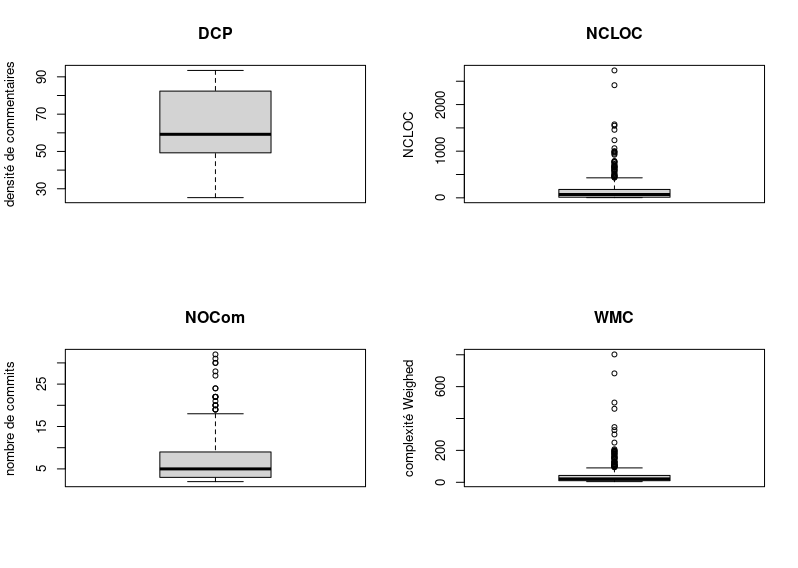
\includegraphics[width=1\columnwidth]{T1.png}
   \end{center}

   \begin{center}
      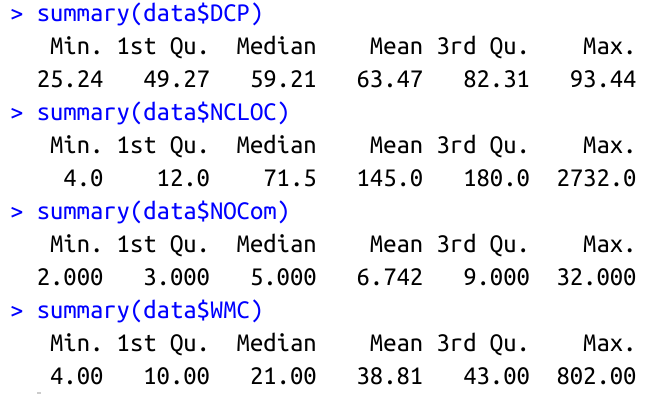
\includegraphics[width=0.6\columnwidth]{T1.1.png}
      \end{center}

   Pour chaque métrique:\\
   NCLOC : nombre de lignes de code qui ne sont pas ni vides ni commentaires \\

   On peut voir qu'il y a beaucoup de points en-dehors du maximum (Potential Outliers). 
   Donc la distributions est asymétrique à gauche.\\
   
   DCP : densité de commentaires (CLOC/LOC) donnée en pourcentage \\
   DCP est un métrique en pourcentage, donc elle est le plus équilibrée.
   La médiane est entre 50\% à 60\%, et il n'y a pas de outliers.  \\

   NOCom : nombre de commits (combien de fois la classe a été changée) dans l’historique git de la classe \\
   On peut voir qu'il y a beaucoup de points en-dehors du maximum (Potential Outliers). 
   Donc la distributions est asymétrique à gauche.\\


   WMC : la métrique de complexité Weighed Methods per Class
   On peut voir qu'il y a beaucoup de points en-dehors du maximum (Potential Outliers). 
   Donc la distributions est asymétrique à gauche.\\
}

 
\end{question}

%----------------------------------------------------------------------------------------
%	QUESTION 2
%----------------------------------------------------------------------------------------

\begin{question}

   \questiontext{T2. (25\%) Évaluer l’hypothèse selon laquelle les classes qui ont été modifiées plus de 10 fois sont mieux
   commentées que celles qui ont été modifiées moins de 10 fois. Décrire d’abord la conception de l’étude et
   discuter par la suite les résultats. Suivez les étapes d’une étude empirique (choix d’étude, énoncé des
   hypothèses, définition des variables, interprétation et généralisation des résultats, discussion des menaces
   à la validité).}
   
   \answer{
      Ici on va évaluer l'échantillon de données pour project jfreechart,
      donc c'est une étude de cas.\\
      L’hypothèse selon laquelle les classes qui ont été modifiées plus de 10 fois sont mieux
   commentées que celles qui ont été modifiées moins de 10 fois. \\
      Des variables:
       On peut utiliser est le DCP car la dictribution de DCP est plus équilibré
     pour mesurer entre des classes.
       On peut aussi utilser le NoCom pour diviser des donnée en deux groupes.\\
      \begin{center}
         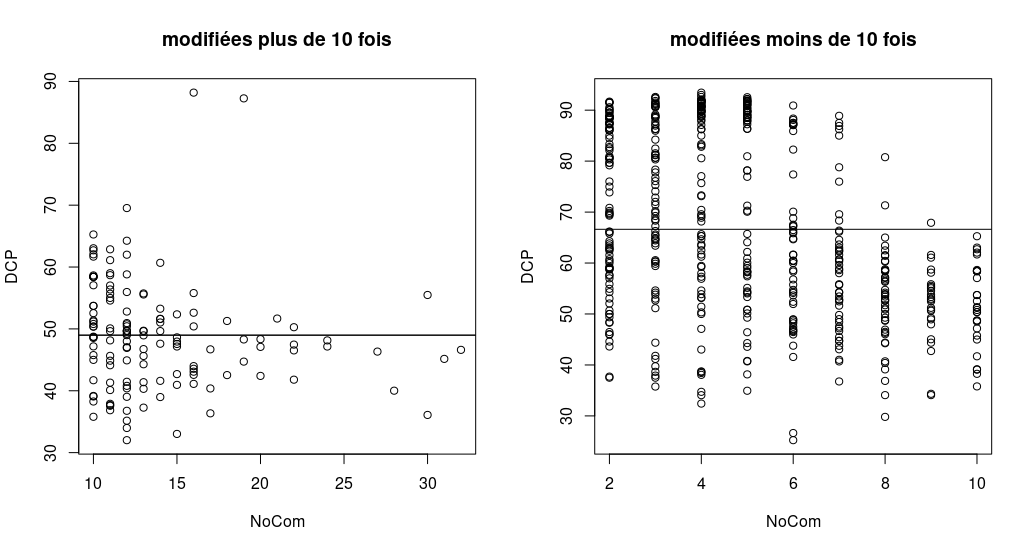
\includegraphics[width=1\columnwidth]{T2.png}
         \end{center}
      On peut voir que la moyenne de DCP des classes qui ont été modifiées 
      moins de 10 fois est plus grand que celles qui ont été modifiées plus de 10 fois. \\
      Donc l’hypothèse pour ce cas n'est pas vraie.\\
      
      Le nombre de classes dans le groupe de moins de 10 fois est de 524. \\
      Le nombre de classes dans le groupe de plus de 10 fois est de 138. \\
      Les deux groupes sont suffisamment grands (>30), donc comparer la moyenne de DCP est bon. 
   
      }
   
    
   \end{question}


%----------------------------------------------------------------------------------------
%	QUESTION 3
%----------------------------------------------------------------------------------------

\begin{question}

   \questiontext{T3. (15\%) Étudier les corrélations entre NCLOC et WMC, DCP et WMC, NOCom et WMC. Visualisez les
   données, les droits de régression, etc., et expliquez pourquoi (ou pourquoi pas) ces visualisations sont
   significatives (ou pas). Dans cette étape, vous ne prenez pas de décisions: vous explorez et vous étudiez
   l'ensemble de données. }
   
   \answer{
      \begin{center}
         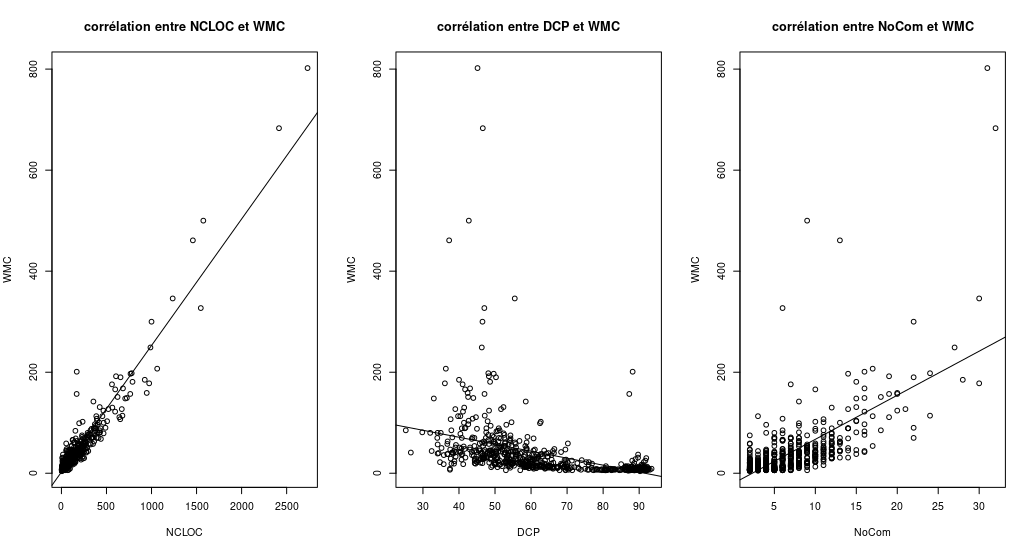
\includegraphics[width=1\columnwidth]{T3.png}
         \end{center}
         La corrélation entre NCLOC et WMC:\\
         L'équation linéaire est : y = 2.4864 + 0.2504*x, correlation entre les deux est 0.9596547.\\
         On peut voir que la corrélation est forte,linéaire et positive, 
         il n’y pas de point de biais, car plus de code de logique, plus de complexité.\\
         
         La corrélation entre DCP et WMC:\\
         L'équation linéaire est : y = 126.477 -1.381*x, correlation entre les deux est -0.3936666.\\
         La corrélation est négative, mais pas si forte, car il y a beaucoup de points de biais, donc la corrélation n’est pas significativement  linéaire.
         La raison est que DCP est en pourcentage.\\

         La corrélation entre NOCom et WMC:\\
         L'équation linéaire est : y = -20.008 + 8.724*x, correlation entre les deux est 0.6626955\\
         On peut voir que la corrélation est forte,linéaire et positive, 
         il y a quelques points de biais, mais la  plupart est autour de la droite, 
         car plus de code de logique sont ajoutés, plus de complexité.\\
   }
\end{question}

%----------------------------------------------------------------------------------------
%	QUESTION 4
%----------------------------------------------------------------------------------------

\begin{question}

   \questiontext{
      T4. (30\%) Évaluer les hypothèses suivantes : \\
      a. WMC est une fonction linéaire du NCLOC \\
      b. WMC est une fonction linéaire du DCP \\
      c. WMC est une fonction linéaire du NOCom \\
      Décrire d’abord la conception de l’étude (comme en T2) et discuter les résultats par la suite. 
   }
   
   \answer{
      a. \\
      Choix d’étude: Étude de cas\\
      Hypothèses: WMC est une fonction linéaire du NCLOC. Afin d'évaluer cette hypothèse nous utilisons la visualisation graphique obtenue à la question 3. \\
      Définition des variables: variable dépendante: WMC; variable indépendante: NCLOC\\
      Discussion des résultats: D'après les résultats obtenus dans cette étude de cas il y a une relation linéaire suggérée entre WMC et NCLOC, l'hypothèse peut donc être acceptée. \\
      \\
      b.\\
      Choix d’étude: Étude de cas\\
      Hypothèses: WMC est une fonction linéaire du DCP. Afin d'évaluer cette hypothèse nous utilisons la visualisation graphique obtenue à la question 3. \\
      Définition des variables: variable dépendante: WMC; variable indépendante: DCP\\
      Discussion des résultats: D'après les résultats obtenus dans cette étude de cas il n'y a pas de relation linéaire significative suggérée entre WMC et DCP, nous pouvons donc rejetter l'hypothèse.  \\
      \\
      c.\\
      Choix d’étude: Étude de cas\\
      Hypothèses: WMC est une fonction linéaire du NOCom. Afin d'évaluer cette hypothèse nous utilisons la visualisation graphique obtenue à la question 3. \\
      Définition des variables: variable dépendante: WMC; variable indépendante: NOCom\\
      Discussion des résultats: D'après les résultats obtenus dans cette étude de cas il y a une relation linéaire suggérée entre WMC et NOCom, l'hypothèse peut donc être acceptée \\
      \\
   }
\end{question}

%----------------------------------------------------------------------------------------
%	QUESTION 5
%----------------------------------------------------------------------------------------

\begin{question}

   \questiontext{
      T5. (5\%) Décrivez vos conclusions dans un court paragraphe. 
   }
   
   \answer{
      Nos résultats se basent sur des études de cas, donc les rélations trouvées, ou non trouvées, sont suggérées et il faudrait faire une expérience ultérieurement afin de les généraliser et ainsi confirmer ou réfuter ces modèles. Nos résultat concluent que la métrique de complexité Weighed Methods per Class (WMC) a une relation linéaire avec le  nombre de lignes de code qui ne sont pas ni vides ni commentaires (NCLOC) et avec le nombre de commits dans l’historique git de la classe (NOCom), mais pas avec la densité de commentaires donnée en pourcentage (DCP). Nos résultat suggèrent que la métrique de complexité Weighed Methods per Class (WMC) a une relation linéaire avec le  nombre de lignes de code qui ne sont pas ni vides ni commentaires (NCLOC) et avec le nombre de commits dans l’historique git de la classe (NOCom), mais pas avec la densité de commentaires donnée en pourcentage (DCP). Il y a un éventail de variables additionnelles qui pourraient avoir une relation avec WMC, mais les variables étudiées étaient celles qui nous étaient fournies. Il reste dans les mains des chercheurs approfondir cettes études de cas pour arriver à des conclusions plus robustes. \\
   }
\end{question}


%----------------------------------------------------------------------------------------
%	QUESTION 1
%----------------------------------------------------------------------------------------

% \begin{question}

% \questiontext{What is the airspeed velocity of an unladen swallow?}

% \begin{center}
% 	\includegraphics[width=0.5\columnwidth]{swallow.jpg} % Example image
% \end{center}

% \answer{While this question leaves out the crucial element of the geographic origin of the swallow,\
% according to Jonathan Corum, an unladen European swallow maintains a cruising airspeed velocity of 
%\textbf{11 metres per second}, or \textbf{24 miles an hour}. The velocity of the corresponding African swallows requires further research as kinematic data is severely lacking for these species.}

% \end{question}


% %----------------------------------------------------------------------------------------
% %	QUESTION 3
% %----------------------------------------------------------------------------------------

% \begin{question}

% \questiontext{Identify the author of Equation \ref{eq:bayes} below and briefly describe it in English.}

% \begin{equation}\label{eq:bayes}
% 	P(A|B) = \frac{P(B|A)P(A)}{P(B)}
% \end{equation}

% \answer{Lorem ipsum dolor sit amet, consectetur adipiscing elit. Praesent porttitor arcu luctus, imperdiet urna iaculis, mattis eros. Pellentesque iaculis odio vel nisl ullamcorper, nec faucibus ipsum molestie. Sed dictum nisl non aliquet porttitor. Etiam vulputate arcu dignissim, finibus sem et, viverra nisl. Aenean luctus congue massa, ut laoreet metus ornare in. Nunc fermentum nisi imperdiet lectus tincidunt vestibulum at ac elit. Nulla mattis nisl eu malesuada suscipit.}

% \end{question}

% %----------------------------------------------------------------------------------------

% \assignmentSection{Bonus Questions}

% %----------------------------------------------------------------------------------------
% %	QUESTION 4
% %----------------------------------------------------------------------------------------

% \begin{question}

% \questiontext{The table below shows the nutritional consistencies of two sausage types. Explain their relative differences given what you know about daily adult nutritional recommendations.}

% \begin{table}[h]
% 	\centering % Centre the table
% 	\begin{tabular}{l l l}
% 		\toprule
% 		\textit{Per 50g} & Pork & Soy \\
% 		\midrule
% 		Energy & 760kJ & 538kJ\\
% 		Protein & 7.0g & 9.3g\\
% 		Carbohydrate & 0.0g & 4.9g\\
% 		Fat & 16.8g & 9.1g\\
% 		Sodium & 0.4g & 0.4g\\
% 		Fibre & 0.0g & 1.4g\\
% 		\bottomrule
% 	\end{tabular}
% \end{table}

% \answer{Lorem ipsum dolor sit amet, consectetur adipiscing elit. Praesent porttitor arcu luctus, imperdiet urna iaculis, mattis eros. Pellentesque iaculis odio vel nisl ullamcorper, nec faucibus ipsum molestie. Sed dictum nisl non aliquet porttitor. Etiam vulputate arcu dignissim, finibus sem et, viverra nisl. Aenean luctus congue massa, ut laoreet metus ornare in. Nunc fermentum nisi imperdiet lectus tincidunt vestibulum at ac elit. Nulla mattis nisl eu malesuada suscipit.}

% \end{question}

% %----------------------------------------------------------------------------------------
% %	QUESTION 5
% %----------------------------------------------------------------------------------------

% \begin{question}

% \lstinputlisting[
% 	caption=Luftballons Perl Script, % Caption above the listing
% 	label=lst:luftballons, % Label for referencing this listing
% 	language=Perl, % Use Perl functions/syntax highlighting
% 	frame=single, % Frame around the code listing
% 	showstringspaces=false, % Don't put marks in string spaces
% 	numbers=left, % Line numbers on left
% 	numberstyle=\tiny, % Line numbers styling
% 	]{luftballons.pl}

% %--------------------------------------------

% \begin{subquestion}{How many luftballons will be output by the Listing \ref{lst:luftballons} above?} % Subquestion within question

% \answer{99 luftballons.}

% \end{subquestion}

% %--------------------------------------------

% \begin{subquestion}{Identify the regular expression in Listing \ref{lst:luftballons} and explain how it relates to the anti-war sentiments found in the rest of the script.} % Subquestion within question

% \answer{Lorem ipsum dolor sit amet, consectetur adipiscing elit. Praesent porttitor arcu luctus, imperdiet urna iaculis, mattis eros. Pellentesque iaculis odio vel nisl ullamcorper, nec faucibus ipsum molestie. Sed dictum nisl non aliquet porttitor. Etiam vulputate arcu dignissim, finibus sem et, viverra nisl. Aenean luctus congue massa, ut laoreet metus ornare in. Nunc fermentum nisi imperdiet lectus tincidunt vestibulum at ac elit. Nulla mattis nisl eu malesuada suscipit.}

% \end{subquestion}

% %--------------------------------------------

% \end{question}

%----------------------------------------------------------------------------------------

\end{document}
